
\chapter{Synthesize: Generalization and Grounding}
\label{ch:haxd}


\begin{figure}[h] %  figure placement: here, top, bottom, or page
   \centering
   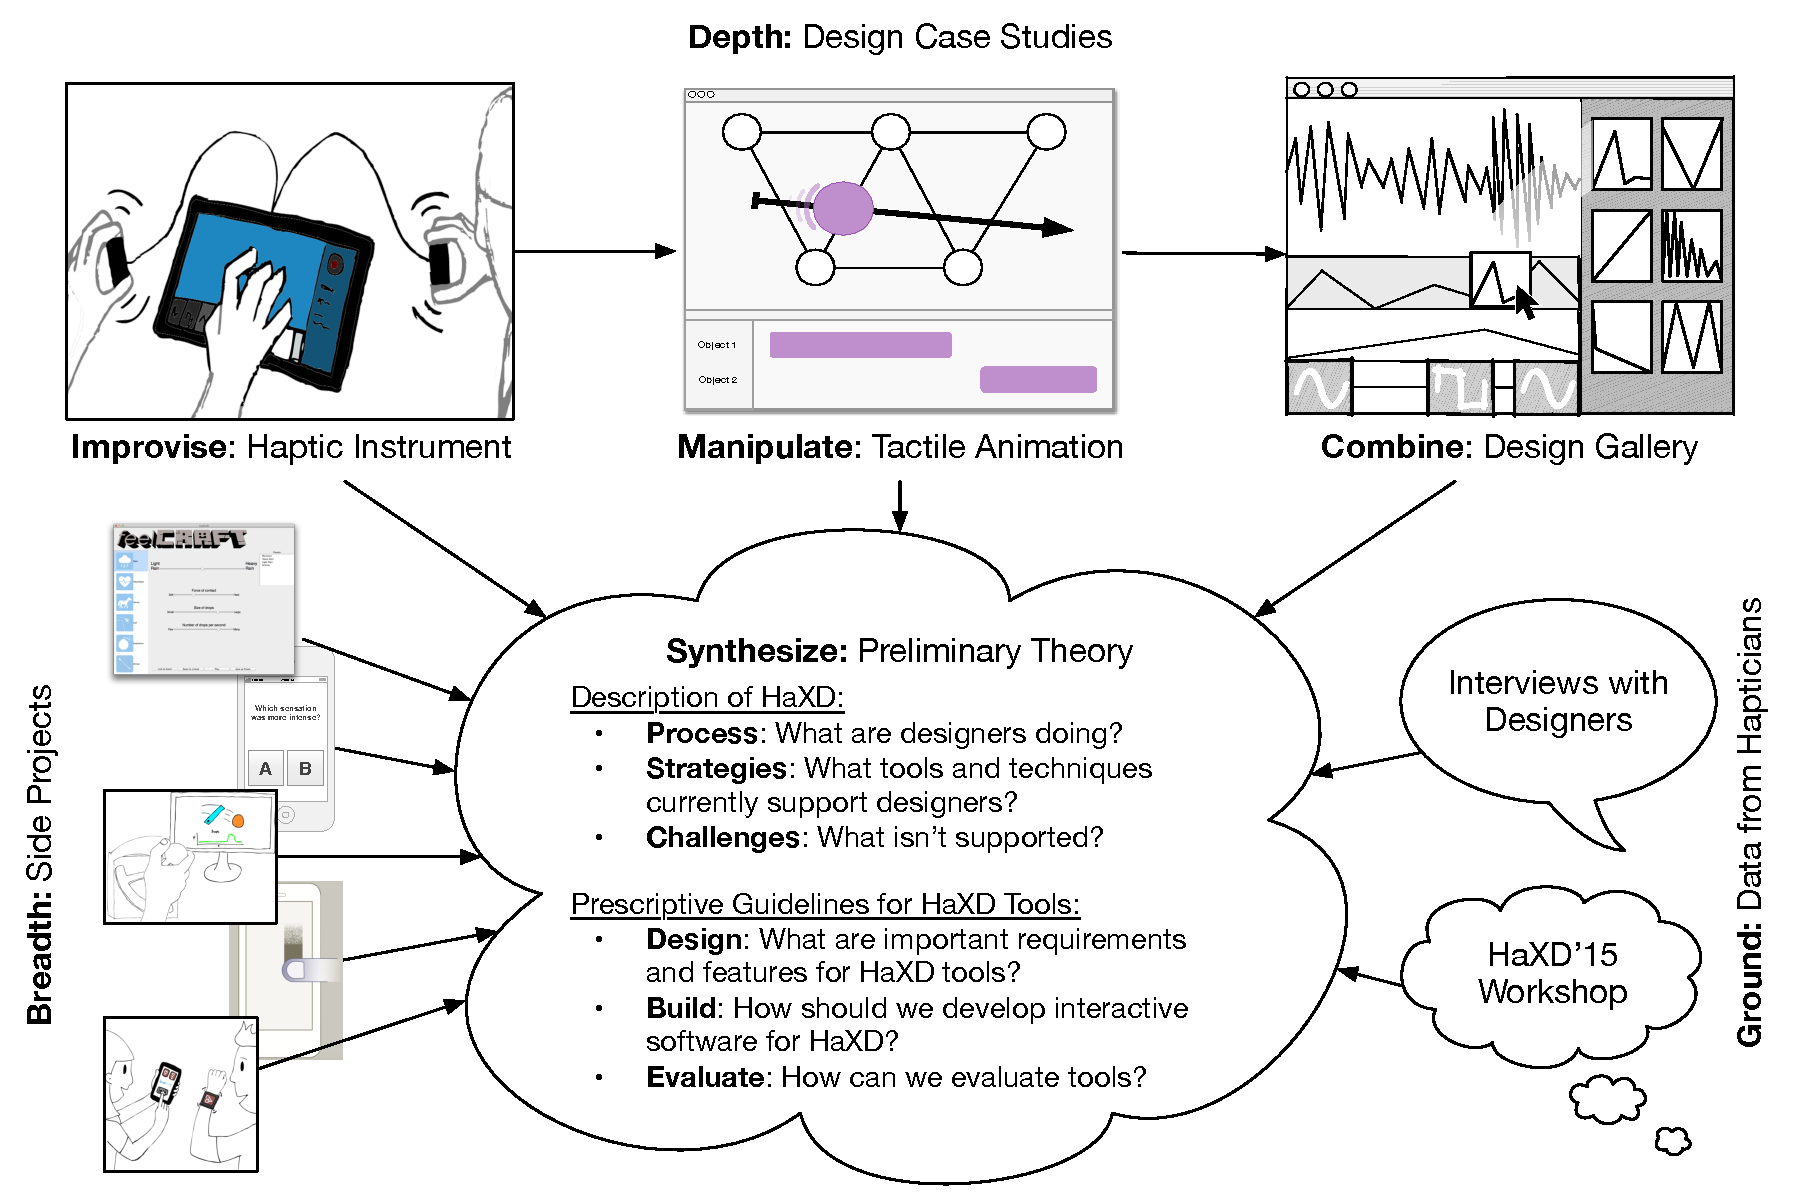
\includegraphics[width=0.7\textwidth]{HaXDTheoryOutline-2015-05-22} 
   \caption{Planned synthesis of data for a preliminary theory of haptic experience design.}
   \label{fig:haxd:theoryoutline}
\end{figure}


The three case studies provide rich but focused data on how to create vibrotactile (VT) experience design tools.
To complement these studies, I propose to gather information more broadly to generalize the haptic design process to other use cases and ground in haptician experience (\autoref{fig:haxd:theoryoutline}).
%from professional haptic designers.
In this way, my final contributions will draw from several sources: 
1) the three in-depth design studies,
%2) a literature survey of general design theories,
2) insight gathered from several side projects, and
3) two sets of grounded data: interviews with professional designers, and
%4) 
%informal interviews with peers at conferences, and 
a workshop at World Haptics `15.

Here, I describe the data collection process, then illustrate possible applications and forms for these contributions.
However, any resulting theory will be emergent from the data, and can take many forms.
To accomplish this in a principled way, I plan to use \emph{memoing} and \emph{constant comparison} \cite{Corbin2008}, looking for common threads between data and double-checking conclusions as new theoretical developments appear.
%This will be guided with a goal: to characterize haptic experience design, especially any features that are unique to this unique class of technological experiences.
This theory will also draw from a literature review of design theory, summarized in this document's related work section.
%This will provide information about non-haptic design disciplines and general theory of design to help frame our inquiry.




%%%%%%%%%%%%%%%%
%
% Section: Data Collection
%
%%%%%%%%%%%%%%%%
\section{Data Collection}
In this section, I list the different sources I intend to use to collect data for theory design.

\subsection{Vibrotactile design case studies}
Each of the  design case studies previously described investigates a specific user group working on a specific VT device with a specific software tool.
Through my experience of gathering requirements, creating tools (through design and development), and evaluating them, I will have first-hand knowledge of supporting aspects of VT sensation design.
Each also produces a small vignette of haptic design in action, giving us glimpses of the design process.

\subsection{Side projects}
In addition to the three design case studies that form this proposal, several side-projects are planned or underway as collaborative efforts.
In these side-projects, I take an organizational or supervisory role, often as summer projects conducted by undergraduates.

\begin{description}
	\item[FeelCraft and Feel Messenger] are collaborations with Disney Research members Ali Israr and Siyan Zhao, looking at distributing and customizing haptic effects in a consumer setting with low-fidelity rumble motor devices.
	I take a haptic designer role to gain a personal understanding of the process, and a software engineer role to understand relevant architectures. % for distributing haptic media.

	\item[CyberHap] is a collaboration between UBC and Stanford looking at force-feedback devices in education; a large team is involved with undergraduate Gordon Minaker leading development of a teaching interface since February 2015, co-supervised by PI Dr. Karon MacLean and me.
%	I co-supervise Gordon with PI Dr. Karon MacLean in this project looking at force-feedback devices in an education setting.
	
	\item[CuddleBit] is a project inspired by the Haptic Creature and CuddleBot project. A small, breathing and vibrating robot will be designed along with a behaviour prototyping tool in summer 2015.
	I supervise undergraduate Paul Bucci in this project exploring multiple modalities and potential for receiving input through a sensor.

	\item[HapTurk] is a collaboration with PhD candidate Hasti Seifi on different techniques to crowdsource feedback on VT icons. Master's student Salma Kashani and undergraduate Matthew Chun are developing visualizations and low-fidelity VT icons during summer 2015.
%	This project looks at a formal mechanism for doing large-scale feedback, and tackles the problem of cross-device and cross-modal equivalency (can a sensation be rendered in some fidelity on both low- and high-fidelity devices?).

	\item[RoughSketch] is a painting application for the TPad Phone, a variable-friction mobile device, for the World Haptics 2015 Student Innovation Challenge. Undergraduates Brenna Li, Paul Bucci, and Gordon Minaker are all fellow team members. Variable friction is a significant contrast to VT sensations as it is intrinsically connected to input: no sensation can be felt without active movement by the user.
\end{description}



\subsection{Grounded Data}
A corpus of interviews with professional haptic designers has already been collected by UBC alumni Colin Swindells during his PhD, but has never been published.
I will analyze these interviews to further ground our findings with real-world haptic designers.

To complement this %, and because professional haptic designers are rare and difficult to find,
we turn to the research community who do design as part of their work.
The planned Workshop on Haptic Experience Design (http://oliverschneider.ca/HaXD) at World Haptics 2015 will also provide a data source.
At this workshop, 4 experts of haptic experience design will speak, participants will reveal their own design challenges in a brainstorming activity, and the ensuing panel discussion should help illuminate practices and paths for future work.

%%%%%%%%%%%%%%%%
%
% Section: Possible Format
%
%%%%%%%%%%%%%%%%
\section{Possible Format}
While the theory can take many forms, I hope to characterize haptic experience design and contrast it with other design fields, especially graphic and audio design.
I hope to find both descriptive and prescriptive results, including current practices, an identification of challenges uniquely facing haptic designers, and guidelines for designers and developers of haptic design support tools.

\subsection{Descriptive Contributions: HaXD Process as Requirements}
My first goal is to describe the \textbf{processes} employed by haptic designers.
This could manifest, for example, as a catalogue of 
existing haptic design tools,
appropriated tools (e.g., using a sound editor to create VT icons),
techniques (e.g., design philosophies like Haptic Sketching),
resources (e.g., libraries and APIs),
platforms (what devices designers are using),
practices in haptics education (undergraduate or graduate level courses),
and tasks undertaken by haptic designers.

For example, to share of haptic experiences, haptic designers create demos
to spread awareness of haptic research and gain feedback from peers.
%One colleague, upon being introduced to the Haptics Symposium conference, said that the haptics community gets demos right.
This is so ingrained into the culture of haptic research that recently a demo-only conference was launched: Asia Haptics.

Once collecting a description of current practices, I expect we might be able to identify \textbf{challenges} and \textbf{strategies} to addressing those strategies, including the ecosystem of available tools: what is working well, and what is broken.
Using our example of collaboration and demos, we might see that in-person demos are effective, but
remote collaboration or asynchronous sharing is challenging. %, but could offer more frequent collaboration between designers.
Available tools include videos and visualizations of demos to explain concepts in lieu of the demo itself.
%Other challenges might include the great variety of different devices, non-haptic tools appropriated for haptic design, the implementation complexity of dealing with hardware, low-level software, and application logic simultaneously, or the strong influence of other modalities (vision, hearing) on perceived touch sensations.

\subsection{Prescriptive Contributions: Guidelines for HaXD Software Tools}
After describing HaXD as a set of requirements, I will then develop guidelines for how to built supportive interactive software tools.
Right now, I plan to organize this into three aspects: how to \textbf{design} tools, including important features relevant to different stages of HaXD; how to \textbf{build} tools, including relevant software architectures and ways to address technical challenges; and how to \textbf{evaluate} tools, methods to capture designer experience and inform future design.

Hypothetical use cases might best explain this contribution.
One examples is using these guidelines for knowledge transfer to industry.
I could use these guidelines to advise or create design software for companies developing haptic hardware platforms (such as the TPad team and UltraHaptics) or software platforms (such as Immersion and Phidgets), bridging the gap from research to industry application.
Another example could be dissemination through haptics education.
Developing a module for a haptic design course, such as CPSC 543, is an accessible way to encapsulate and test these ideas.
This could also manifest in a multi-day workshop, similar to Camille Moussette's Haptic Sketching workshops, to validate ideas at different institutions.



\section{Deliverables and Risk}
There are two expected deliverables from this theory development.
First, the HaXD'15 workshop on Haptic Experience design is planned, piloted, and scheduled for World Haptics in June, 2015. 
To get the most out of this workshop, photographs and notes will be recorded.
Afterwards, a very small digest piece debriefing the workshop is planned in winter 2016; this may be submitted on its own as an short paper if an appropriate venue is available (e.g., a special journal issue similar to \cite{Jones2014}), or subsumed into the second deliverable.

The second deliverable is a retrospective piece on our findings from all the data sources found here, but with a focus on data from haptic designer interviews.
This interview data has already been collected by UBC alumnus Colin Swindells.
I plan to digest and analyze those interviews in winter 2016 to generate requirements grounded in designer experience.
This will likely be combined with synthesized findings from the three design studies and several side projects.
To mitigate risk, we can combine interview findings to a greater or lesser extent with other data sources.
If the interviews have a great deal of information, they could be a valuable contribution on their own.
If not, I expect them to supplement our other data sources.
This document will likely be submitted as a full paper to a peer-reviewed conference or journal.

Within each project, we mitigate risk through strategic planning and study design;
many of these projects do not have to be successful to provide input.
For example, HapTurk may never actually be deployed, but could still articulate the challenge of a large-scale, remote haptic user study.
In addition,
risk is partially managed through sheer attrition: one or two side projects or data sources could provide limited feedback and we would still have a diverse set of information. 
However, I will note that initial investigation has already been useful.

%
%To ground our other findings with our target end users, and identify challenges that may not emerge from the literature alone.
%The goal is to develop an initial proposed theory of haptic experience design from multiple sources, which characterizes the unique process that can or could support designers.
%I plan to gather information from a variety of sources, including interviews with professional designers, informal interviews with peers during conferences, and the literature.


%The main source of data will be from interviews with professional designers, several of which have been collected already by researcher Colin Swindells.
%These will be analyzed using qualitative techniques like grounded theory and phenomenology \cite{Creswell2013, Moustakas1994}.
%
%A second source of data will be reflection on our own projects and those of our peers and collaborators.
%
%
%Currently, much of the literature review has already been conducted for this document, 
%





%% KM - for comments
%\newcommand{\inlinecomment}[3][]{$\lceil$\textbf{#1}~\textit{\textcolor{#2}{#3}}$\rfloor$}
%\definecolor{DarkGreen}{rgb}{0.0, 0.5, 0.0}
%\definecolor{DarkRed}{rgb}{0.7, 0.2, 0.2}
%\definecolor{DarkOrange}{rgb}{1, 0.5, 0}
%\definecolor{Orange}{rgb}{1, 0.75, 0}
%\newcommand{\kmC}[1]{\noindent \inlinecomment[KM]{DarkGreen}{#1}}
%\newcommand{\kmE}[1]{\textcolor{DarkRed}{#1}}
%\newcommand{\osC}[1]{\noindent \inlinecomment[OS]{Orange}{#1}}
%%\newcommand{\osC}[1]{}
%\newcommand{\osE}[1]{\textcolor{DarkOrange}{#1}}
%
%%Organization commands
%\newcommand{\inlineHeading}[1]{\emph{#1} --}
%
%%\newcounter{pathwayCounter}
%\newcommand{\challenge}[1]{\textbf{Pathway: #1} --}
%
%
%Although haptic technologies have become commonplace in end-user experiences, there are still few established processes to guide designers, who face special challenges that arise out of the relative youth of the field and from qualities intrinsic to the sense of touch.
%Design guidelines, toolkits, and authoring interfaces exist as disparate pieces of knowledge rather than a unified perspective, 
%hobbling the creativity and efficiency needed to create new haptic experiences. 
%In this paper, we assemble key elements of the haptic design process and its
%needs
%into a generalized
% framework and vocabulary, 
%to promote
% a more fluid, extendable, and transferrable understanding of the practice, 
%guide development of effective tools, and 
%promote a discourse around both. 
%We begin with haptic versions of three primary
% design activities identified in
% design theory, creativity support tools, and other fields of design: problem preparation, hands-on design, and collaboration.
%These activities form a framework by which we can organize the haptic design literature and our own experience 
%into specifically defined
%pathways for design, identifying areas for future research and implications for tool development.
%
%
%
%
%\begin{table*}
%\caption{Design Activities, Sub-Activities, and Pathways Synthesized from the Literature}
%\label{tab:designactivities}
%
%%
%%
%%% Old version - horizontally laid out
%%
%%\begin{center}
%%	\begin{tabular}{|c|c|c|c|c|c|c|c|c|}
%%	\hline
%%		
%%		
%%	\multicolumn{3}{|c|}{\bf Problem Preparation (\Cref{sec:problempreparation}) }
%%		& \multicolumn{3}{|c|}{\bf Hands-on-Design (\Cref{sec:handsondesign})}
%%		& \multicolumn{3}{|c|}{\bf Collaboration (\Cref{sec:collaboration})} \\
%%		
%%		\multicolumn{3}{|c|}{\emph{Use the Designer's Experience}}
%%		& \multicolumn{3}{|c|}{\emph{Navigate a Design Space}}
%%		& \multicolumn{3}{|c|}{\emph{Design together}} \\
%%		
%%	\hline
%%		
%%	Framing
%%		& Repertoire
%%		& Examples
%%	& Ideation
%%		& Evaluation
%%		& Sketching
%%	& Relate
%%		& Feedback
%%		& Donate \\
%%		
%%	%sub-activities
%%	\emph{Defining}
%%		& \emph{Internal}
%%		& \emph{External}
%%	& \emph{Generation}
%%		& \emph{Filtering}
%%		& \emph{Rapid, flexible,}
%%	& \emph{Informal talks}
%%		& \emph{Formal studies}
%%		& \emph{Dissemination} \\
%%		
%%	\emph{the problem}
%%		& \emph{experience}
%%		& \emph{resources}
%%	& \emph{of ideas}
%%		& \emph{of ideas}
%%		& \emph{ambiguous notation}
%%	& \emph{with peers, mentors}
%%		& \emph{with users}
%%		& \emph{to community} \\
%%		
%%%	\hline	
%%%	%Challenges
%%%	\emph{Flexible interfaces,}
%%%		& \emph{Accessible}
%%%		& \emph{Example}
%%%	& \multicolumn{2}{|c|}{Support multiple}
%%%		& \emph{Support ambiguity,}
%%%	& \multicolumn{3}{|c|}{Challenge: \emph{investigate asynchronous,}} \\
%%%		
%%%	\emph{multiple views}
%%%		& \emph{knowledge}
%%%		& \emph{management}
%%%	& \multicolumn{2}{|c|}{parallel designs}
%%%		& \emph{commenting, abstraction}
%%%	& \multicolumn{3}{|c|}{ \emph{distributed collaboration}} \\	
%%		
%%	\hline
%%	\end{tabular}
%%\end{center}
%%\end{table*}
%%
%
%
%\begin{center}
%	\begin{tabular}{lll}
%	\toprule
%		
%
%%	\rowcolor [gray]{.8}
%	\textbf{Activity}
%		& \textbf{Sub-Activity}
%		& \textbf{Pathways for Design}
%		\\
%	\midrule
%	
%	\multirow{3}{1.7in}{\textbf{Problem Preparation (\Cref{sec:problempreparation})} \emph {Use the Designer's Experience}}
%		& Framing -- Defining the problem
%		& Flexible interfaces, multiple views, powerful language
%		\\
%	\cmidrule{2-3}
%		& Repertoire -- Internal experience
%		& Task-based knowledge source
%		\\
%	\cmidrule{2-3}
%		& Examples -- External resources
%		& Manage examples: capture, find, access, transform
%		\\
%	\midrule
%	
%	\multirow{3}{1.7in}{\textbf{Hands-on Design (\Cref{sec:handsondesign})} \emph {Navigate a Design Space}}
%		& Ideation -- Generate ideas
%		& \multirow{2}{*}{Explore multiple design candidates in parallel}
%		\\
%	\cmidrule{2-2}
%		& Evaluation -- Filter ideas
%		&
%		\\
%	\cmidrule{2-3}
%		& Sketching -- Rapid, flexible, ambiguous notation
%		& Support speed, ambiguity, commenting, abstraction
%		\\
%	\midrule
%	
%	
%	\multirow{3}{1.5in}{\textbf{Collaboration (\Cref{sec:collaboration})} \emph {Design Together}}
%		& Relate -- Informal talks with peers, mentors
%		& \multirow{3}{*}{Explore asynchronous and distributed interactions}
%		\\
%	\cmidrule{2-2}
%		& Feedback -- Formal studies with users
%		&
%		\\
%	\cmidrule{2-2}
%		& Donate -- Dissemination to community
%		&
%		\\
%	
%		
%%	\multicolumn{3}{|c|}) }
%%		& \multicolumn{3}{|c|}{\bf Hands-on-Design (\Cref{sec:handsondesign})}
%%		& \multicolumn{3}{|c|}{\bf Collaboration (\Cref{sec:collaboration})} \\
%%		
%%		\multicolumn{3}{|c|}{\emph{Use the Designer's Experience}}
%%		& \multicolumn{3}{|c|}{\emph{Navigate a Design Space}}
%%		& \multicolumn{3}{|c|}{\emph{Design together}} \\
%%		
%%	\hline
%%		
%%	Framing
%%		& Repertoire
%%		& Examples
%%	& Ideation
%%		& Evaluation
%%		& Sketching
%%	& Relate
%%		& Feedback
%%		& Donate \\
%%		
%%	%sub-activities
%%	\emph{Defining}
%%		& \emph{Internal}
%%		& \emph{External}
%%	& \emph{Generation}
%%		& \emph{Filtering}
%%		& \emph{Rapid, flexible,}
%%	& \emph{Informal talks}
%%		& \emph{Formal studies}
%%		& \emph{Dissemination} \\
%%		
%%	\emph{the problem}
%%		& \emph{experience}
%%		& \emph{resources}
%%	& \emph{of ideas}
%%		& \emph{of ideas}
%%		& \emph{ambiguous notation}
%%	& \emph{with peers, mentors}
%%		& \emph{with users}
%%		& \emph{to community} \\
%		
%%	\hline	
%%	%Challenges
%%	\emph{Flexible interfaces,}
%%		& \emph{Accessible}
%%		& \emph{Example}
%%	& \multicolumn{2}{|c|}{Support multiple}
%%		& \emph{Support ambiguity,}
%%	& \multicolumn{3}{|c|}{Challenge: \emph{investigate asynchronous,}} \\
%%		
%%	\emph{multiple views}
%%		& \emph{knowledge}
%%		& \emph{management}
%%	& \multicolumn{2}{|c|}{parallel designs}
%%		& \emph{commenting, abstraction}
%%	& \multicolumn{3}{|c|}{ \emph{distributed collaboration}} \\	
%		
%	\bottomrule
%	\end{tabular}
%\end{center}
%\end{table*}
%
%
%
%
%%%%%%%%%%%%%%%%%%%%%%%%%%%%%%%%%%%%%%%%%%%%%%%%%%%%%%%%%%%%%%%%%%%%%%%%%%%%%%%%%
%\section{Introduction}
%Haptic technology has become a 
%standard ingredient of user interactions with technology, with the potential to add engagement to media experiences \cite{Modhrain2001, Danieau2014} and ``calm'' everyday interactions \cite{MacLean2009}.
%% No longer restricted to research labs or theme park rides, 
%Carefully designed and expressive haptic feedback is finding its way into commercial devices, most recently the Apple Watch (www.apple.com/watch).
%
%
%
%\begin{figure}[tbp] %  figure placement: here, top, bottom, or page
%	\centering
%	\begin{subfigure}[b]{0.23\textwidth}
%		   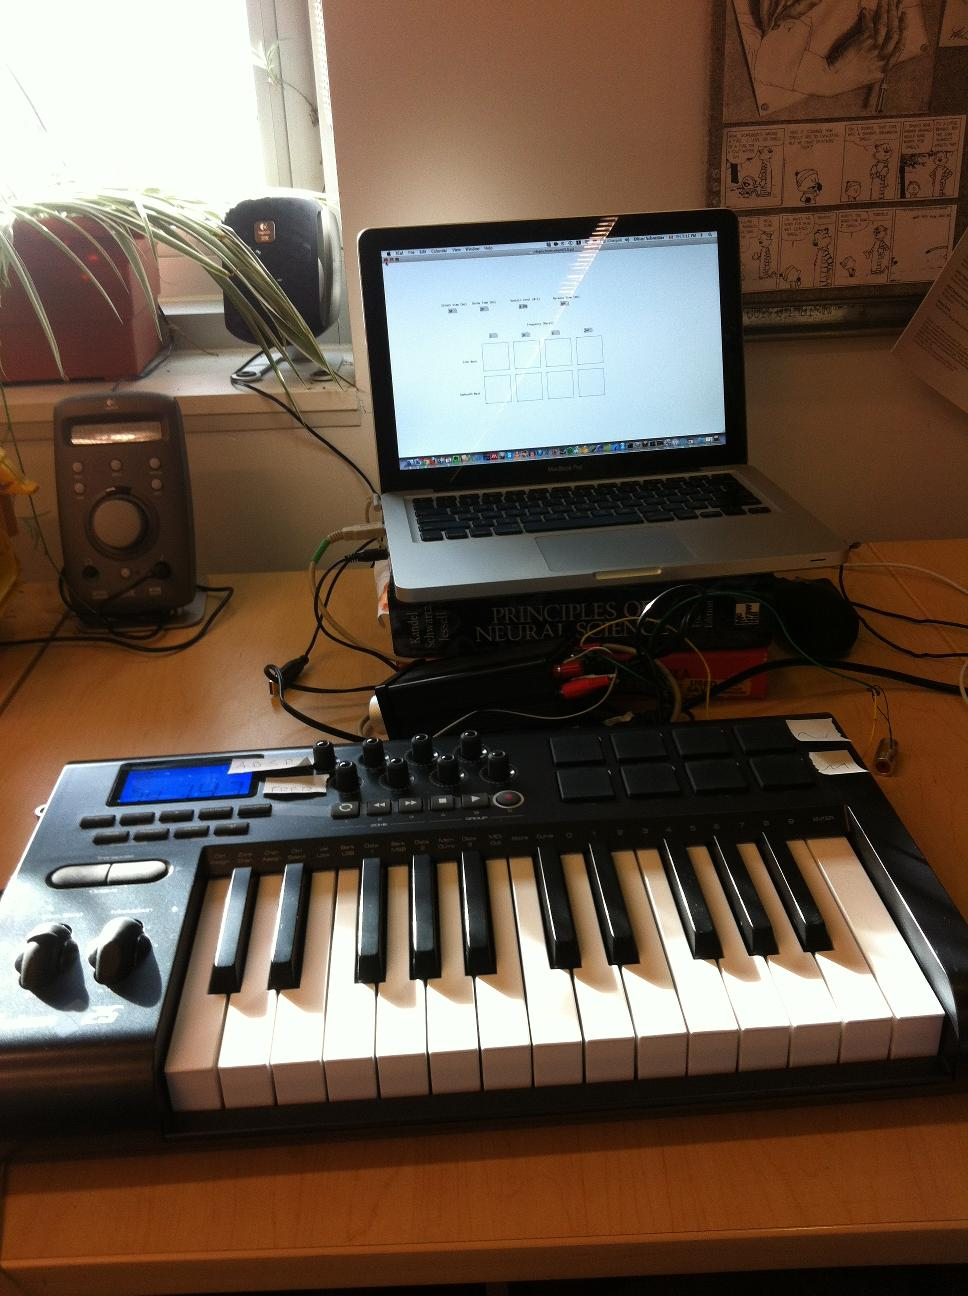
\includegraphics[height=2.3in]{figures/HIVE-photo} 
%		   \caption{Early hardware sketch}
%		   \label{fig:example:hardware}
%	\end{subfigure}
%	\quad
%	\begin{subfigure}[b]{0.22\textwidth}
%		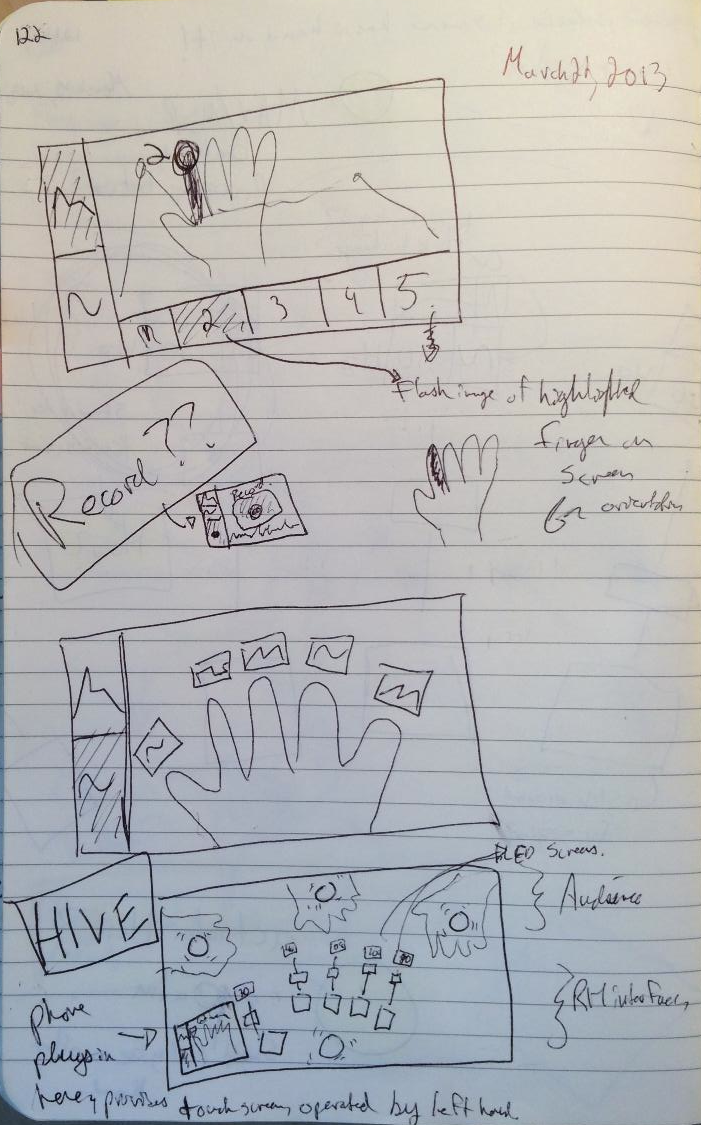
\includegraphics[height=2.3in]{figures/mHIVE-earlysketch-photo-cropped} 
%		\caption{Early paper sketch}
%		\label{fig:example:paper}
%	\end{subfigure}
%	\caption{Early sketches for mHIVE \cite{Schneider2014} in hardware (a) and on paper (b), showing a \emph{framed} approach (instrument metaphor), inspiration from the designer's \emph{repertoire} (musical experience), and extension of \emph{examples} (dials and buttons adapted from the keyboard).}
%	 \label{fig:example}
%\end{figure}
%
%
%% Despite this growth, 
%Nevertheless, there is no established process for haptic experience design (``HaXD").
%% (HaXD) %OS: We never reuse this, but may want to in future drafts
%% has no established design process.
%% One culprit is the small and fragmented user base:
%Culprits abound. The user base is small and fragmented:
%professional haptic designers are still rare, often share engineering or scientific duties, and tend to be sequestered in companies whose business needs preclude broader interactions % with other designers.
%and complicate observation of design practices by researchers.
%%\kmE{They lack both training in an articulated user-experience design approach, and an interlinked community through which they can consolidate vocabulary and share best practices.}
%It is difficult to translate guidelines from other fields, in absence of analogies to % graphic design's 
%colour % theory 
%or musical theory. % for touch.
%Designing for the sense of touch entails % brings intrinsic design challenges, such as  %as it involves 
%hard-to-prototype hardware and context-sensitive perception~\cite{Hayward2008}.
%
%%However, when attempting to get that ineffable quality of getting something to ``feel right" in a given context, a robust design process can help when prescriptive guidelines fail.
%
%Recently, design thinking applied to haptics \cite{Moussette2012} has added to the literature on HaXD process \cite{Swindells2006}.
%Toolkits \cite{Minamizawa2012,Ledo2012}, effect libraries \cite{Israr2014},  collaborative software \cite{Ruthenbeck2014,Cha2009} and interfaces themselves \cite{Schneider2014} ease production of haptic \emph{effects}.
%However, a systematic, convergent procedure by which haptic \textit{experiences} can be developed
%to meet specific requirements -- which themselves may be hard to articulate -- is elusive, % not well defined, 
%with previous work providing only % isolated elements. % 
%pieces of the puzzle.
%
%In this paper, we aim to situate
%haptic design tasks in a common framework.
%Synthesizing insights from design and creativity literature, we describe
% three critical activities conducted during many types of design: 
% \textit{problem preparation}, \textit{hands-on design}, and \textit{collaboration}, each with
% sub-activities.
%We discuss each in the haptic context to discover what activities are supported and which are not,
%with examples drawn from literature and our personal experience as designers and observers of other designers.
%This design lens
%reveals not only a process, but pathways for more focused investigation, informing the creation of HaXD support tools.
%
%
%
%%\inlineHeading{Design Activities}
%
%
%%\begin{table}
%%\caption{Problem Preparation Sub-Activities}
%%\label{tab:problem:preparation}
%%\begin{center}
%%	\begin{tabular}{|l|p{2cm}|p{2cm}|p{2cm}|}
%%	\hline
%%		&Description	&Haptics so far	& Haptics next	\\
%%	
%%	
%%%	\hline
%%%	\textbf{Problem Preparation}	&	&	&	\\
%%	
%%		\hline
%%		\emph{Framing}
%%			& transforming the problem into a manageable form
%%			& Ongoing investigation of haptic language, perceptual dimensions
%%			& Flexible, adaptable tools; multiple views	\\
%%
%%		\hline
%%		\emph{Repertoire}
%%			& building the designer's internal experience
%%			& Haptics education (e.g., HapKit,  Twiddler), DIY haptics, haptic illusions
%%			& Handbook, wiki, or other more elaborate compendium of knowledge	\\
%%		\hline
%%		\emph{Examples}
%%			& Drawing from external resources and designs
%%			& Haptic camera, libraries (Immersion, Upenn, FeelEffects), haptic search engine
%%			& Capture \& upload, find (search/explore/visualize), use (design galleries, editable data types)	\\
%%	\hline
%%	\end{tabular}
%%\end{center}
%%\end{table}
%
%
%
%%\subsection{Challenge: Difficult Problem Framing}
%%The CHALLENGES (unfilled holes):
%%
%%1. Problem Gathering:
%%No Language, limited theory (framing)
%%Complex sense (hard to understand, need to be expert in multiple domains
%%) (repertoire+framing)
%%No language/theory
%%limited ways to capture, render, maintain examples
%
%
%\challenge{Multiple metaphors}
%Despite a steady progression of research on perception,
%there is no agreed upon language for working with haptics \cite{Obrist2013,Okamoto2013,Jansson-Boyd2011}.
%Most authoring tools have relied on fixed metaphors and devices, limiting \emph{framing}.
%Allowing  multiple metaphors or views on a haptic design is one way in which a designer can % would allow the designer to 
%reshape a problem to be easier to solve (reframe it so it matches their \emph{repertoire} or found \emph{examples}).
%Future authoring tools should pursue flexibility or improved abstractness.
%%Abstract metaphors could apply to multiple device classes, .
%
%%Examples:
%%?	Haptic Camera
%%?	Kuchenbecker?s haptic textures
%%?	Libraries
%%?	Feel Effects/FeelCraft
%%?	Ultrasound Examples from Keisuke Hasegawa?s HaptoMime at AsiaHaptics:
%%o	Tried a bunch of waveforms extracted from sound sources in the Komplete audio packagewith my own palm. It?s a pity that there was no systematic procedure to determine what waveform to pick up. My only advice is that it would be good and efficient to construct an experimental system which allows you to test many kinds of stimuli promptly at an early stage in y our researches.
%%?	Need examples from industry
%
%
%
%%\kmC{Isn't this a library not an education problem? SLC} % Not following the focus on haptics education here, as related to repertoire. Can you strengthen the connection? I thought this particular challenge would be more about how designers can capture, organize, find, reuse externally sourced inspiration and examples - essentially, the library problem. Education, and communication with one another, is an important but different challenge.}
%% That said, I am still fuzzy on distinction between repertoire and examples. They both need libraries, don't they? Because there are a lot of them, and the point is re-use. 
%\challenge{Task-based knowledge}
%To build their \emph{repertoire}, haptic designers must learn essential haptics concepts and begin solving relevant problems.
%Haptics courses \cite{Okamura2012, Jones2014} often provide a HaXD practitioner with initial experience.
%Brief, cogent outlines  of haptics knowledge (e.g., \cite{Hayward2007,MacLean2008,Hayward2008,Karam2013}) allow designers to expand their experience in an accessible way, and resources like EduHaptics (eduhaptics.org) link designers to content.
%However, knowledge is still framed with disparate perspectives. 
%The next step is to understand the low-level tasks conducted in HaXD.
%This would enable development of a more focused ``how-to" compendium of knowledge uniting perception, hardware, and software knowledge bases.
%%Ideally, this will link directly to HaXD tasks, but more research is needed to understand the .
%%, but still accessible, source of knowledge; a handbook of haptics knowledge that summarizes perceptual research, lists prominent examples of design, and guidelines for design and development.
%%This need not be a traditional handbook, but could be an online tool, such as a wiki or online course.
%%A proposed handbook might have more content internalized, structured to be handy and self contained, featuring design case studies.
%
%%\emph{Examples}
%\challenge{Manage examples}
%Currently, \emph{examples} exist in several libraries (e.g., \cite{Culbertson2014, Israr2014}), but capturing, organizing, accessing, and transforming them poses a greater challenge for haptic design than for more visually oriented, or even auditory, domains.
%%Excluding progress made by expanding these libraries in scale or in device support, there are key areas we can look for future progress.
%Capturing with a haptic camera  \cite{MacLean1996} is useful, but limited to that camera's target phenomenon.
%Integration of library uploads into authoring tools (e.g., as suggested in \cite{SchneiderAsiaHaptics2014}), would make it easier to grow a set of \emph{examples}.
%Visualizations, searching techniques (like a haptic search engine \cite{Adi2010,Hanamitsu2014}), and browsing techniques will facilitate access.
%%One demoer at a recent conference described his approach to create a tactile effect.
%%He tried waveforms extracted from sound sources in the Komplete audio package, stating ``It's a pity that there was no systematic procedure to determine what waveform to pick up" and wishing for a system to try stimuli at an early stage.
%%with my own palm. It?s a pity that there was no systematic procedure to determine what waveform to pick up. My only advice is that it would be good and efficient to construct an experimental system which allows you to test many kinds of stimuli promptly at an early stage in y our researches.
%%In haptics, we have already done some work on capturing examples, for example, the haptic camera \cite{MacLean1996}, or empirically gather libraries \cite{Culbertson2014}.
%% Some examples or templates are often shipped with toolkits (Verify!), and recently vibrotactile libraries have been developed: Immersion, Feel Effects, or the UPenn surface toolkit \cite{Culbertson2014}.
%%The haptic search engine (asia haptics) is one way of recalling examples.
%Finally, current \emph{examples} are static -- the designer chooses one and adds it to their application.
%%Novel techniques of using examples to create new designs.
%Open, manipulatable formats beyond parameters (like those in \cite{Ledo2012,Israr2014}) or through design galleries \cite{Lee2010a,Marks1997} is an exciting avenue to allow designers to work hands-on with \emph{examples}.
%
%%Originating in the graphics literature, design galleries provide a set of designs similar or different from your current design, letting users take interesting parameters and apply them to their design \cite{Marks1997}.
%%This idea has since been applied to other design fields like web design \cite{Lee2010a}.
%%Given the difficulty of framing with no fixed haptic parameters or language \cite{Jansson-Boyd2011}, example-based design could be a promising avenue for future design tools.
%%It's also been recommended that focusing on rapid prototyping can get around language barriers in haptics \cite{Fogg1998}.
%%To do this, we need to focus on hands-on design of haptics, the second major design activity.
%
%
%
%%Rapid iteration is essential for being able to think by doing; creativity support tools must have a low threshold, high ceiling, and wide walls: accessible to beginners, powerful for complete solutions, and support a wide range of explorations \cite{Resnick2008}.
%%A sketch can have many purposes, but is distinguished from a prototype by being more generative, less complete, and characteristic of earlier design \cite{Buxton2007}.
%
%
%
%
%%Donald Sch\"{o}n's seminal book, The Reactive Practitioner, describes the process of
%%learning skills to be one of reflection-in-action. That is, a pitcher in a baseball game must be able to find their groove. Through a process of subtle adjustment and experimentation, a pitcher adjusts her technique to fit the current, myriad conditions the wind, the current batter, the sun; the list goes on. This process is implicit, and often people find it impossible to articulate. Like the poor centipede, we sometimes find it difficult to realize that knowledge is embedded in our action, and in fact it can ruin our stride. Verbal overshadowing, articulating a wine's taste or a person's face, often weakens our memory unless we've been trained to verbalize those notions \cite{Schooler1990}. Similarly, a haptic designer must adapt to her design project to the current conditions.
%
%%Idea generation vs Idea evaluation. Sketching.
%
%
%%\begin{figure}[htbp] %  figure placement: here, top, bottom, or page
%%   \centering
%%   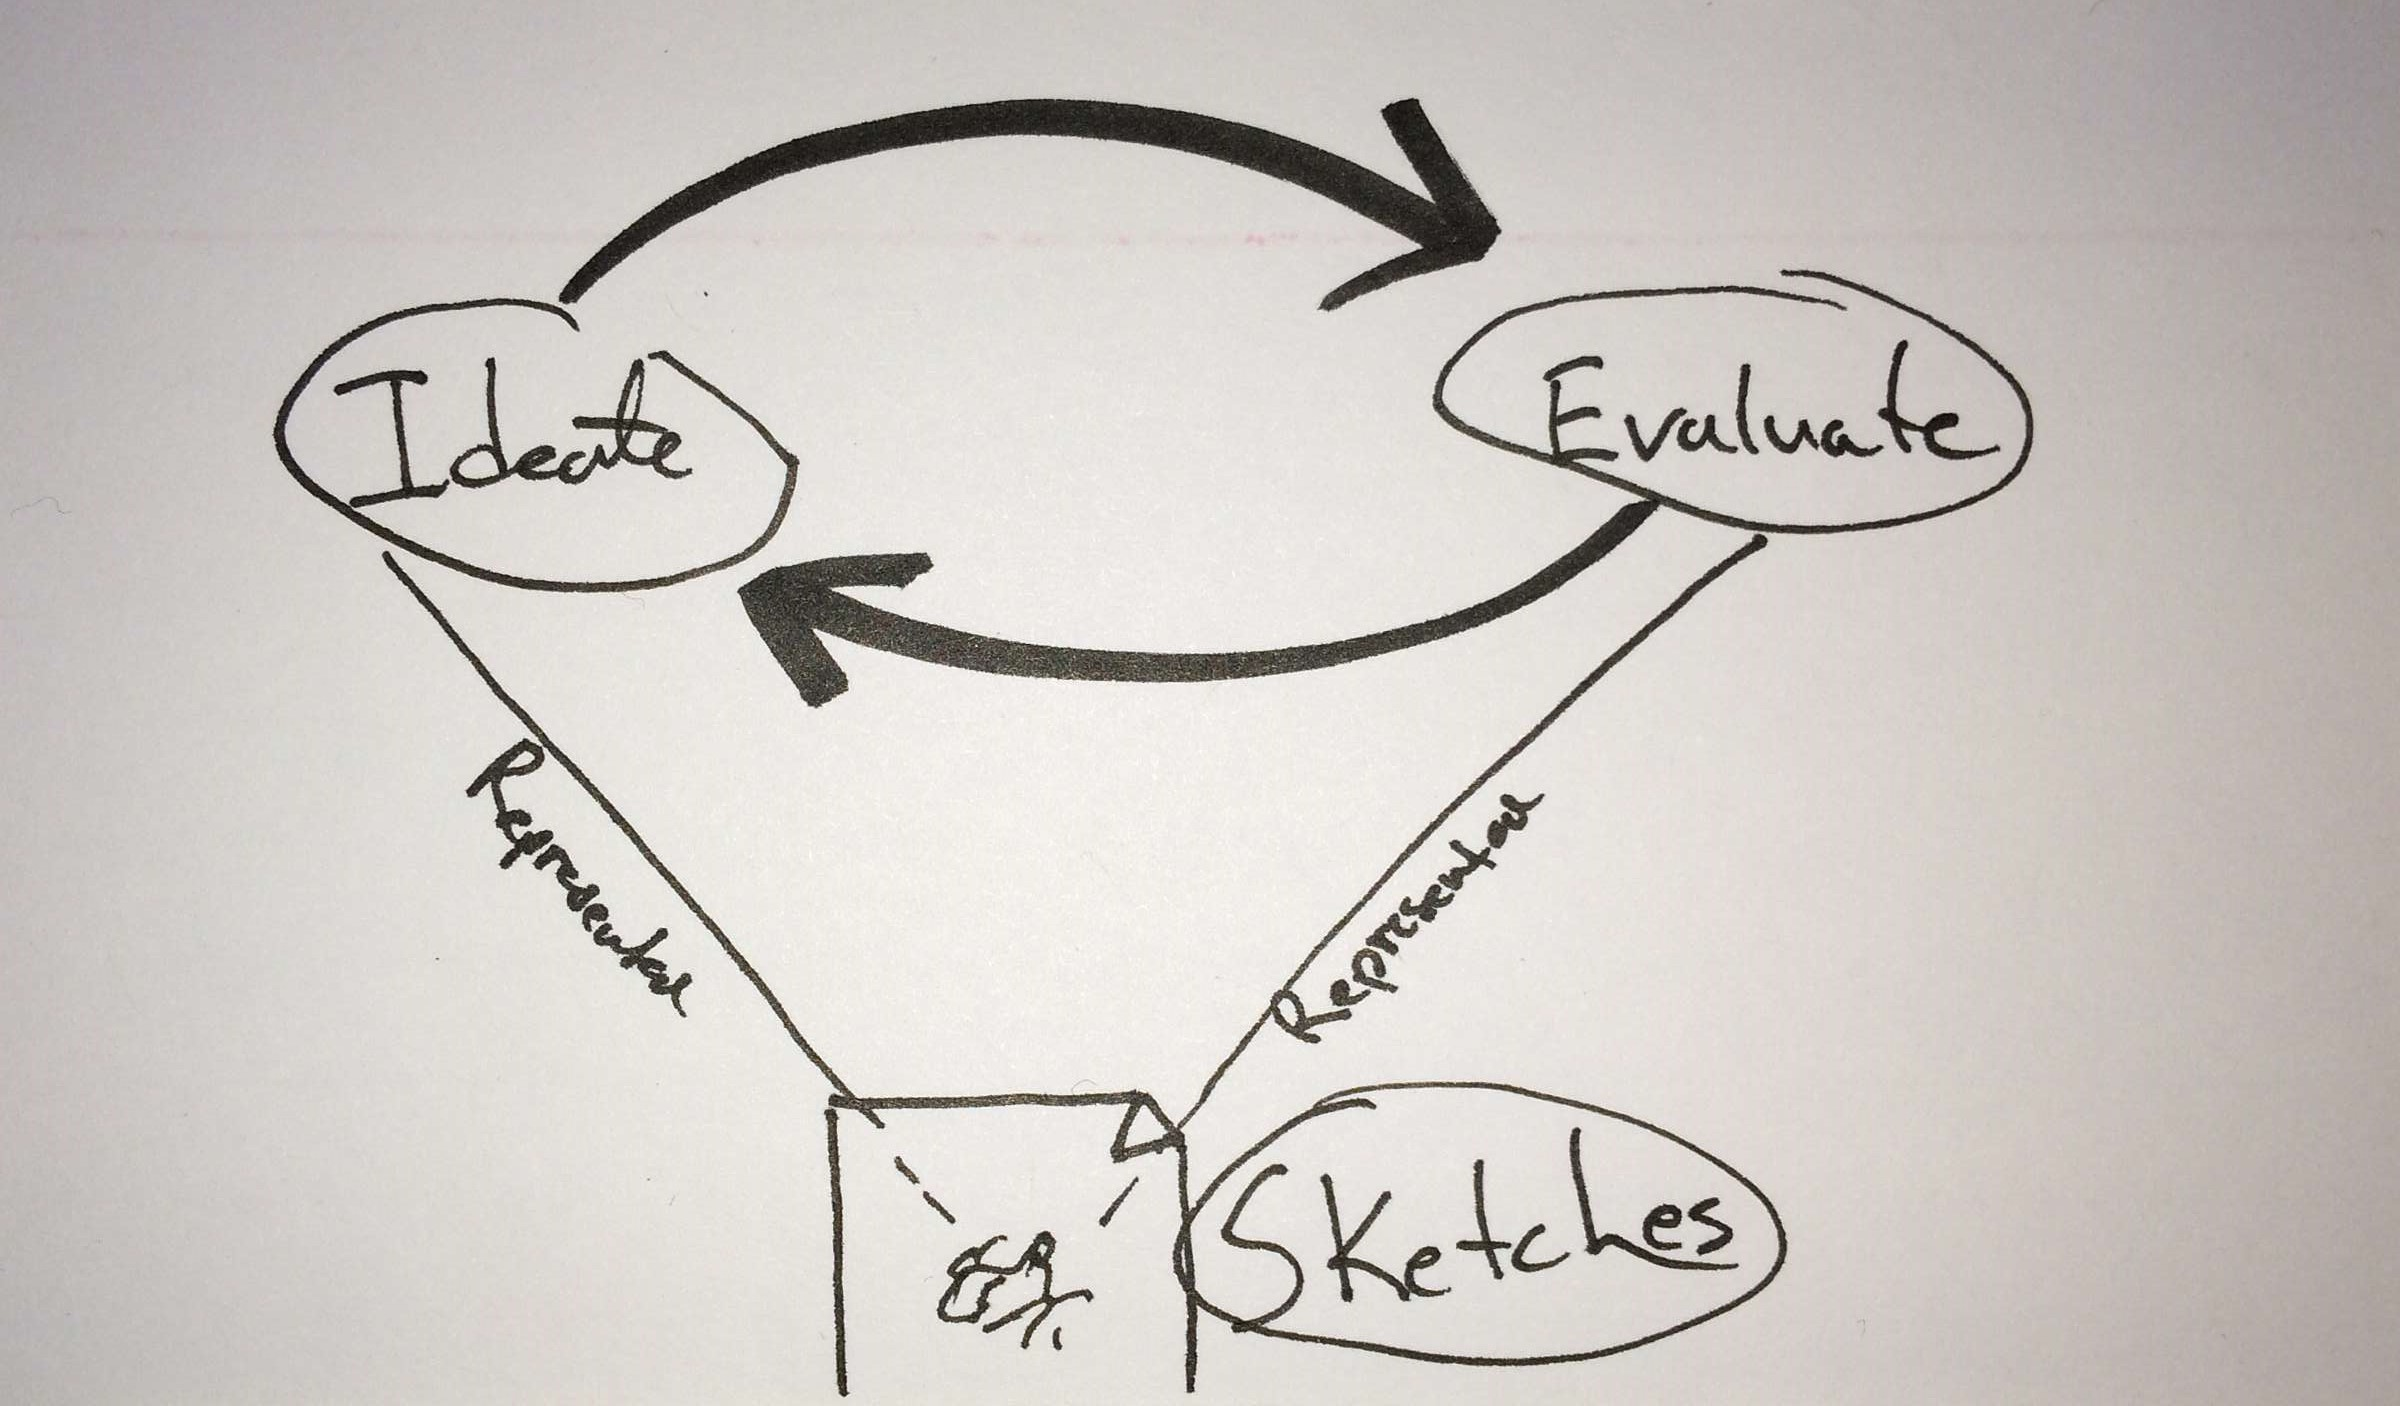
\includegraphics[width=0.48\textwidth]{figures/HandsOnDesignSubProcessesPlaceHolder} 
%%   \caption{Hands-on design sub-activities. Designers iterate between ideation and evaluation, representing this process through sketches.\textbf{(PLACEHOLDER)}}
%%   \label{fig:hands:on:sub:activities}
%%\end{figure}
%
%
%\challenge{Multiple, parallel designs}
%Ideation and evaluation are partially supported by existing tools.
%Parallel development of interfaces has been applied to physical UIs with Arduino \cite{Hartmann2008}.
%Brainstorming and techniques like A/B testing, comparing two designs side-by-side, have been employed in haptics design tools \cite{Swindells2014}.
%Rapid ideation and evaluation are also supported through better framing tools like design galleries, described in the previous section.
%
%\challenge{Ambiguity, commenting, \& ad-hoc use}
%%Haptic design suffers from slow iteration.
%%Developing a haptic sensation often requires custom hardware, software, and coordination between the two.
%%Further, other senses must be considered, meaning a full stack of hardware to high-level GUI software must be developed and maintained.
%Haptics, involving software and hardware, can require time to iterate.
%Haptic sketching prioritizes rapidly exploring ideas through physical sketches \cite{Moussette2011,Moussette2012}.
%%Sketchinghas been explored recently with haptic design.
%%Sketches are  conducted with whatever material is at hand, often using only lightweight programming or no programming at all.
%Interfaces that capture the spirit of sketching have been shown to support real-time feedback \cite{Hong2013, Schneider2014}.
%%Toolkits provide support for certain tools, but inhibit flexibility and ambiguity, key aspects of sketching.
%While the community is working to use rapid development with more, sophisticated hardware setups, 
%sketching requires other features to be truly useful.
%Ambiguous sketches show only necessary detail or relevant view points, helping a designer work with half-formed ideas questions. %problems, and supports initial framing to final refinement.
%Unfortunately, a haptic sensation requires a physical implementation, which must be exactly specified.
%Good defaults or randomized tools might be valuable - allow designers to specify constraints they understand, and let other details be filled in automatically.
%Sketching should also support annotation and editing -- circling problem areas, writing down related ideas -- and ad-hoc use.  
%With a pen, any napkin is a canvas. Haptics needs napkins too.
%% To truly support brainstorming and feedback, however, collaborative design must be considered.
%
%%Supporting a mobile context with compact tools could benefit sketching.
%
%%\emph{Ideation and Evaluation}
%
%
%
%%%%%%%
%% Groupware design space
%%%%%%%%
%\begin{table*}[ht]
%\centering
%	\caption{Collaboration Sub-Activities Across Groupware Dimensions}
%	\label{tab:collaboration}
%	
%	\begin{tabular}{lccc}
%	
%	%\cmidrule{2-4}
%	\multicolumn{1}{l}{} & \textbf{Relate} & \textbf{Feedback} & \textbf{Donate} \\
%	
%	\midrule
%
%	Face-to-Face 
%		& \emph{Informal demo}
%		& \emph{Typical user study}
%		& \emph{Demo}
%		\\
%	\midrule
%	Asynchronous
%		& \emph{Installation \& commenting system}
%		& \emph{Self-running user study}
%		& \emph{Demo installation}
%		\\
%	\midrule
%	Distributed Synchronous
%		& \emph{Video chat with two devices}
%		& \emph{User study-at-a-distance}
%		& \emph{Live broadcast}
%		\\
%	\midrule
%	Distributed Asynchronous
%		& \emph{Email, wikis, source code management}
%		& \emph{Crowd sourced study}
%		& \emph{Tutorials, haptic video}
%		\\
%	\midrule
%	\end{tabular}
%
%\end{table*}
%
%
%%Examples:
%%Haptic Sketching (Moussette)
%%Haptic Instrument
%%Need some maker culture examples
%%NEED HAPTICS EXAMPLES/ANECDOTES FROM DEMOs
%
%%	
%%		
%%		\hline
%%		\textbf{Hands-on Design} &	&	&	\\
%%		
%%		\hline
%%		\emph{Idea generation}
%%			& \emph{todo}
%%			& \emph{todo}
%%			& \emph{todo} \\
%%		
%%		\hline
%%		\emph{Idea evaluation}
%%			& \emph{todo}
%%			& \emph{todo}
%%			& \emph{todo} \\
%%			
%%		\hline
%%		\emph{Sketching}
%%			&Ambiguous, rapid representations of ideas at varying levels of abstraction
%%			& Haptic sketching (Moussette), 3Doodler (Kickstarter), Haptic Instrument (Schneider \& MacLean), Demonstration based tool (Choi's lab)
%%
%%			& Ambiguity, abstraction, annotation \\
%%		
%%		
%%		\hline
%%		\textbf{Collaboration}&	&	&	\\
%%		\hline
%%		\emph{Relate}
%%			& Frequent, informal feedback from colleagues, peers, family, friends
%%			& Already the case in collocated, synchronous situations
%%			& Expand to distributed or asynchronous collaboration \\
%%			
%%		\hline
%%		\emph{Donate}
%%			& Sharing a creation with the general world; publishing it
%%			& We can write and provide pictures/videos; some file formats for given tool kits
%%			& Need ways to be able to share haptics more generally; publishing mechanism that works on different devices (or provides the "gist" of a haptic effect)\\
%%			
%%		\hline
%%		\emph{Feedback}
%%			& User studies, experiments, and other ways of more formal feedback
%%			& There's a lot of experiments done and written up to be replicable; some authoring tools (Swindells)support A/B testing
%%			& Expand to asynchronous, distributed feedback (mechanical turk and other crowd sourced platforms); add streamlined framework for experiements (right now most are custom built, but maybe they have to be)
%%	\\
%
%%
%
%
%
%
%
%%Larger movements in force-feedback devices can be shared by video, e.g., demonstrating instability.
%%Smaller actuation, such as skin stretch, vibrotactile devices, and
%
%
%%Collocated asynchronous - installations like the Lega, where tactile impressions attach to art exhibits, felt by mobile device \cite{Laaksolahti2011}
%
%%\kmC{what about device generalization? May have missed. Also a prototyping challenge}
%
%
%%%%%%%
%% Groupware dimensions
%%%%%%%%
%%\begin{table}
%%\centering
%%	\caption{Groupware Dimensions}
%%\kmC{this table needs to do more work, or be dropped - SLC}
%%%  It's been often-published, so consider carefully whether it merits the space here as opposed to a single sentence description. It would be more valuable if you could add haptics-relevant detail to each of the 4 cells?
%%	\label{tab:groupware}
%%	
%%	\begin{tabular}{r|l|l|}
%%		\multicolumn{1}{r}{} & \multicolumn{1}{c}{Same Time} & \multicolumn{1}{c}{Different Times} \\
%%		\cline{2-3}
%%	Same Place & Face-to-face  & Asynchronous  \\
%%		\cline{2-3}
%%	Different Places & Synchronous distributed  & Asynchronous distributed  \\
%%		\cline{2-3}
%%	\end{tabular}
%%
%%\end{table}
%
%
%
%
%%Examples:
%%Sile Modhrain haptic broadcasting -> donating
%%MPEG5 -> donating
%%Haptic Instrument, FeelCraft
%%Haptic cinematography?
%%NEED MORE
%%One example is Cyberhap – the problem of verifying remote kits have been assembled correctly.
%
%%\section{Haptic Challenges for Design}
%%Each of these 3 design activities are important to use in haptic design, however,  they are difficult to accomplish. In this section, we describe N challenges specifically related to haptics, and how they impact each of the 3 design activities.
%%
%%\textbf{Treat this section as a series of LEMMAS for challenge section, or, roll into challenges (next section)}
%%
%%
%%
%%\subsection{Touch is a complex sense}
%%Non-localized, fusion of multiple senses (tactile, kinesthetic), influenced by other sense (vision, audio) and other cognitive processes (attention, emotion?).
%%
%%
%%
%%
%%
%%
%%
%%%Framing
%%%-	designers must have an understanding of this complicated sense
%%%-	complex to model examples
%%%-	
%%%Hands-on
%%%-	??
%%%Collaboration
%%%-	???
%%
%%
%%\subsection{Context}
%%Individual differences, multimodal effects, attention (merge with touch as a complex sense)?
%%
%%%Framing
%%%-	???
%%%Hands-on
%%%-	??
%%%Collaboration
%%%-	Hard to match the design environment to that which is shared (donation, evaluation)
%%%-	Example: Allison Okamura and the Stanford
%%
%%
%%\subsection{Many Device paradigms}
%%The technological dual to Challenge 1 (Touch is a Complex Sense), the devices we use for actuation vary dramatically. Unlike graphics, where we have an established pipeline resolving to a 2-dimensional matrix of colour values, and audio, where  a waveform is eventually rendered (possibly in multiple channels for surround sound), there is no standard paradigm. Every device is necessarily different, as it has a different physical mechanism.
%%Traditionally, haptic devices are separated into force-feedback devices and tactile output, roughly corresponding to proprioception and tactile mechanoreceptors. Both of these paradigms require a different rendering model, with force feedback devices typically real-time virtual environments, while tactile devices are simpler. Within these two classes of devices, paradigms still vary - skin stretch devices [] may require different rendering pipelines than vibrotactile mechanisms. Finally, complexity compounds when multiple devices are used, such as skin stretch with force feedback [cite Okamura lab demo?], multiple devices.
%%The resulting challenge for designers is that, for almost any output device, the designer has to think in a different way, and has to enable the necessary infrastructure – load the right software, etc.. If a switch ever needs to be made to another device, this incurs heavy costs, meaning a device decision must be chosen early and, quite possibly, without feeling the fully developed result.
%%There are paradigms that have an established or possibly simple output paradigm (namely, 3 degree-of-freedom force feedback devices like the Phantom or Falcon), but this only represents one class of output device; this is exactly the challenge that haptic designers and their supporters must face.
%%
%%Framing
%%-	Designers must change their framing for every device they work with, making it difficult to work on multiple projects, transfer knowledge from previous projects on different devices, or organize their data/deliverables.
%%Hands-on
%%-	Simply trying out an idea to choose a device becomes a serious investment. Designers are locked into a platform early on, making it hard to convince stakeholders that, force feedback really isn’t working for an application but a skin stretch device would be better.
%%Collaboration
%%-	???
%%
%%
%%\subsection{Complexity}
%%Not only are there many device paradigms, each one needs software, communication protocols, and different ways of interacting with the control flow of the application. Architectural decisions, like choosing whether to have server, client, or mixed control, must be made for every application case and limit generalization. Similar to the Multiple Device challenge, this adds to initial startup costs, meaning rapid ideation or dramatic changes are challenging. Hardware is often custom or in active development. Ultimately, to create a haptic experience, designers must consider everything from hardware, control and rendering techniques, perceptual considerations, communication protocols, software architecture, GUIs and other multimodal concerns, and the overall experience in spite of that. A full stack needs to be created or maintained when creating a haptic experience, slowing iteration.
%%
%%Framing
%%-	Because of the complexity of running a haptic system, the designer may not be able to change their model for design. Data types need to be shared between different levels of the system, hardware is difficult to swap out.
%%Hands-on
%%-	It’s difficult to try out ideas rapidly, as implementations need to be fully described (sketching relies on partial description)
%%-	Changes to a design are either slow and error prone (if complexity is not handled well), or incur significant initial time and effort constraints (if complexity is handled well at the beginning). If custom software is needed, designers must choose whether to have flexibility or to try ideas out quickly early in the design.
%%Collaboration
%%-	Adding support for collaboration adds additional complexity. Eliciting feedback often needs logging (a cross-cutting concern difficult to add to a system [cite aspect-oriented design]) or multiple versions (something only rarely addressed in today’s software systems [cite juxtapose]); networking for distributed systems only increases complexity.
%%-	Donation can be challenging as well, as a correct build environment needs to be established
%%-	Relation is actually kinda supported well if people are collocated, as you can invite colleagues to try your demo when it works (ignoring the perceived “demo effect” where things break down when you show them to an audience).
%%
%%
%%\subsection{Tight technical bounds}
%%1kHz, mechanical control, synchronized with other multimodal output
%%
%%Framing
%%-	???
%%Hands-on
%%-	??
%%Collaboration
%%-	???
%%
%%
%%\subsection{No language or theory}
%%There is no way to talk about haptics, either linguistically, visually, or … . Also
%%In Mindstorms [4], Seymour Papert tells the story of Jim:
%%Consider the case of a child I observed through his eighth and ninth years. Jim was a highly verbal and mathophobic\footnote{Papert uses the term ``mathophobic" for two overlapping concepts: a fear of mathematics (especially
%%in a school environment), and more generally a fear of learning (especially a fear of one or more specific
%%subjects because of a preconception of ineptitude). In this case, he is favouring the first meaning.} child from a professional family. His love for words and for talking showed itself very early, long before he went to school. The mathophobia developed at school. My theory is that it came as a direct result of his verbal precocity. I learned from his parents that Jim had developed an early habit of describing in words, often aloud, whatever he was doing as he did it. This habit caused him minor difficulties with parents and preschool teachers. The real trouble came when he hit the arithmetic class. By this time he had learned to keep “talking aloud" under control, but I believe that he still maintained his inner running commentary on his activities. In his math class he was stymied: He simply did not know how to talk about doing sums. He lacked a vocabulary (as most of us do) and a sense of purpose. Out of this frustration of his verbal habits grew a hatred of math, and out of the hatred grew what the tests later confirmed as poor aptitude.
%%With adult experts in a field, we can assume that they do not lack a purpose. This leaves the vocabulary as a major obstacle, a vernacular of touch that enables us to more clearly talk and think about haptic sensation.
%%Framing
%%-	No language or theory to thinking in when framing the problem
%%-	Hard to organize examples, search them
%%-	
%%Hands-on
%%-	Structuring hands-on transformations is challenging
%%Collaboration
%%-	Can’t talk about haptics, either with collaborators (relating) or providing feedback (evaluation)
%%
%%
%%\subsection{No Cultural idioms}
%%Combine with language/theory point above? Example: There’s no pinch-to-zoom style idiom that’s familiar. Also, no visual idioms beyond waveforms.
%%
%%Repertoire
%%-	??
%%Framing/Problem Definition
%%-	???
%%Hands-on
%%-	??
%%Collaboration
%%-	???
%%
%%
%%\subsection{Perceptual and Meaning dimensions aren't understood}
%%Still establishing what perceptual dimensions there are
%%
%%Repertoire
%%-	??
%%Framing/Problem Definition
%%-	???
%%Hands-on
%%-	??
%%Collaboration
%%-	???
%
%
%
%
%%\section{Designing Haptic Experiences}
%%With these concepts in mind, we review work made to supporting haptic experience design.
%%Through the design lens, we can see progress on some fronts, and outline next steps for future research.
%
%
%\section{Discussion}
%In this section, we illustrate the value of this framework in two ways: articulating scope for a hypothetical tool (``haptic mechanical turk"), and general design implications for a haptic authoring interfaces.
%
%1) Haptic mechanical turk is a hypothetical scenario where Mechanical Turk users can participate in a vibrotactile perception study.
%The users download a mobile app and respond to vibrations, then the app sends the data back to a experimental server.
%This project targets a distributed, asynchronous system to gather \emph{feedback} on vibrotactile sensations.
%It articulates one pathway through the design space, sidestepping some known challenges but confronting others:
% there is no need for synchronous communication or collocated interaction, for problem preparation or hands-on design.
% This guides the HaXD process, presenting device generality as the (non-trivial) problem to be solved.
% %This leaves just device generality as the (sadly non-trivial) problem to be solved,  guiding our process
%
%2) The pathways naturally inform design guidelines, each one advising how to support its corresponding activity.
%For example, we suggest that a haptic design tool should have multiple views, each corresponding to a different mental model (\emph{framing});
%have good default values to support ambiguous specification of sensations (\emph{sketching});
%and have a publishing system in place to distribute sensations (\emph{donate}).
%%So what's the upshot of seeing haptics through the design lens?
%%It....
%%\textbf{todo:} \emph{Here I want to propose two or three projects that are made easier by a good task definition. For example, haptic mechanical turk (like, distributing a VT study over mechanical turk) to support distributed, asynchronous feedback. This is the money section, showing what this framework can do}.
%
%%\textbf{Summarize previous section, synthesize together a little bit} into THINGS THAT ARE GOOD and THINGS THAT ARE BAD AND NEED TO BE IMPROVED; it's a little split up in the previous section
%%
%%Much remains to be done to support the design of haptic experiences.
%%Although perhaps intimidating, there is hope.
%%Progress has been made on isolated fronts.
%%Our hope is that, by applying a design lens to haptics, we can identify new paths for progress that could facillitate the transfer of haptics from research labs to commercial applications.
%%
%%Indeed, haptics practitioners are uniquely strengthened by these challenges.
%%Cross documents the idea of ``design thinking", noting that designers operate seamlessly across different levels of abstraction, from high-level systemic goals to low-level physical properties \cite{Cross2011}.
%%In a recent meeting with interdisciplinary experts, our software engineering colleague was amazed at the way haptics researchers flitted from low-level concerns (USB bandwidth and protocols) to high-level goals (brainstorming interaction design), describing it as giving him a sense of vertigo.
%%With a little inspiration drawn from other design fields, we can turn these obstacles into a unique strength to create a new wave of user experiences.
%
%
%\section{CONCLUSION}
%
%In this paper, we presented a framework of activities important for haptic experience design (HaXD), which organizes previous work into a united perspective, provides a vocabulary for design discourse, and illuminates pathways for future research and tools. 
%In future work, we plan on validating this proposed framework in two ways.
%First, we plan on adopting it in our own work, using it to help define future studies, and using those studies to amend or expand this framework.
%Second, we plan on looking to professional designers to provide empirical validation and improvement of the model.
%This is the first step towards a validated model of haptic design tasks and body of knowledge on how to support those tasks through design tools.
%Right now we have proposed a model, now the task is to validate it and also to use it to support the design of engaging haptic experiences.
%




\endinput
